% -----------------------------------------------
% Template for FA2025 Proceedings

% DO NOT MODIFY THE FOLLOWING SECTION!!
%-------------------------------------
\documentclass[11pt]{article}
\usepackage{fa2025}
\usepackage{amsmath}
\usepackage{cite}
\usepackage{url}
\usepackage{graphicx}
\usepackage{color}
\usepackage{siunitx}
\usepackage[utf8]{inputenc}
%-------------------------------------

% Title.
% ------
\title{Individual violin sound identification \\ using audio features and machine learning}

% Note: Please do NOT use \thanks or a \footnote in any of the author markup

% Three addresses
% --------------
\threeauthors
  {Hugo Pauget Ballesteros} {Institut d'Alembert \\ {\tt hugo.pauget@dalembert.upmc.fr}}
  {Philippe Lalitte} {IReMus \\ {}}
  {Claudia Fritz} {Institut d'Alembert \\ {}}
% ------------

\sloppy % please retain sloppy command for improved formatting
\begin{document}

\maketitle
\begin{abstract}
Identifying individual instruments of the same type from their recordings is a rarely addressed challenge. This paper explores violin sound identification using two datasets of recordings, featuring multiple violinists playing multiple violins. Several long-term audio features were compared, and their performance in violin classification was evaluated using classical machine learning algorithms. Among these features, long-term MFCCs demonstrated the ability to distinguish individual violins while taking into account player-induced variability, enabling reliable violin recognition. Additionally, the influence of key parameters -- such as the number of violinists and choice of musical excerpts -- on classification performance was analyzed. These findings offer guidelines for optimizing future data collection aimed at capturing a violin's unique sound signature.
\end{abstract}
\keywords{\textit{violin identification, classification, features}}
%

\section{Introduction}\label{sec:introduction}
Musical instrument classification is a key task in Musical Information Retrieval (MIR), aiming to identify the instruments present in a recording. This topic has been extensively studied in the literature, and for monophonic recordings (containing only one instrument), state-of-the-art models commonly reach accuracies of almost 100\%. 
However, few articles have addressed the issue of identifying individual instruments of the same type, and even less so when focusing specifically on instruments from the violin family.
Only a handful of studies (\cite{lukasik2010, wang2020, yokoyama2022a}) have tackled this challenge. These studies suggest that cepstral coefficients offer enough discriminative information about individual violin timbre for effective classification. Nevertheless, these studies relied on limited datasets, where not all violins were played by multiple violinists. This raises an important question: do these algorithms recognize the instruments themselves, or simply the unique playing styles of the performers?

\noindent This paper aims to address this challenge by reviewing and comparing various approaches to identify individual violins, from data collection to processing. It provides guidelines for recording sessions and introduces a long-term adaptation of MFCCs. The paper is organized as follows: section \ref{sec:methodology} describes the methodology, including data collection, feature extraction, data exploration, and classification using machine learning. The experimental results are presented and analyzed in section \ref{sec:results}. Finally, section \ref{sec:conclusions} provides concluding remarks and outlines potential directions for future work.


\section{Materials and Methods}\label{sec:methodology}

\subsection{Datasets}
Two datasets were collected for this study, each consisting of recordings where a group of violinists played a set of violins. The violins and violinists sets were different in those two experiments. The first dataset includes a larger number of violins and violinists, while the second dataset comprises more recording time.

\subsubsection{Bilbao Dataset}
During the Bilbao Project, thirteen violins were built to relate their material and geometrical characteristics with their tonal quality \cite{fritz2019a}. These violins were played in 2019 by twenty-three professional violinists, each of them having recorded a 3-octave G chromatic scale on each violin and a short musical excerpt on a violin of their choice. The resulting dataset comprises $13 \times 23$ recordings of scales and $23$ recordings of musical excerpts (one excerpt per violinist). The recordings were made under the same conditions in a large rehearsal room at the Bilbao conservatory, keeping a constant distance between the player and the microphone (Zoom H4n Pro) and using a sample rate of 48kHz.

\subsubsection{CNSM Dataset}
Another dataset was created at the Paris Conservatoire (CNSMDP), involving thirteen violinists and three violins. Participants were given time to familiarize themselves with each instrument before recording a chromatic scale and selected excerpts from the classical violin repertoire. These excerpts were taken from pieces by Bach, Mozart, Tchaikovsky, Sibelius, and Glazunov. The recordings were made under the same conditions in a large recording studio at the CNSM, keeping a constant distance between the player and the microphone (DPA 4006) and using a sample rate of 48kHz.

\subsection{Features}

\subsubsection{Long-Term Average Spectra (LTAS)}
The Long-Term Average Spectra (LTAS) of a recording is obtained by dividing the input signal into overlapping segments, then calculating the windowed DFT of each segment and finally averaging the power of those DFTs.

\noindent LTAS has been used in \cite{buen2005} to compare the tonal quality of violins. More specifically, the author compared the sound of old Italian violins (Stradivari/Guarneri) and modern violins. He concluded that differences between these two groups could be demonstrated using LTAS


\subsubsection{Long-Term Cepstral Coefficients (LTCC)}
LTCC were introduced in \cite{lukasik2010} for individual instrument identification. Their calculation is similar to that of MFCCs (see next section) except that a mel-filterbank is not applied and that the final step is given by an Inverse Discrete Fourier Transform.

\subsubsection{Mel-Frequency Cepstral Coefficients (MFCC)}

MFCCs are obtained by mapping the frequencies of a spectrum onto a nonlinear mel-scale (a perceptual scale of pitches judged by listeners to be equal in distance from one another), taking the logarithm, and then computing the Discrete Cosine Transform (DCT) of the result. Here, instead of calculating the MFCCs on overlapping segments, we use an LTAS as input spectrum as we want features with a long-term meaning.

\noindent MFCCs are a set of features that has been extensively used for Automatic Speaker Recognition and for Instrument Classification (e.g. \cite{eronen2000, deng2008}).

\subsection{Classifiers}
We compare the results of three popular classification algorithms : K-Nearest Neighbours, Support Vector Machines and MultiLayer Perceptron. These three classifiers use different learning strategies and thus will give different results on our data.

\section{Results and Discussions}\label{sec:results}

This section analyses classifier performance for violin identification. First, we provide an overview of the performance achieved by different features and classifiers, followed by the introduction of a fine-tuned baseline model. Subsequently, the influence of key hyperparameters on the performance of this baseline model is systematically examined. The results highlight the impact of dataset subsets and hyperparameter configurations on model effectiveness, offering insights into optimal settings for violin identification tasks.

\subsection{Model performance}

We first compare the performance of various features and classifiers. For each combination, we systematically tuned hyperparameters to determine optimal configurations. As our datasets are small, we use a repeated random sub-sampling cross-validation to compute the accuracy of each model. The best performing model is then selected as our baseline. The results of this comparative analysis are summarized in figure \ref{fig:accuracy-bilbao} for the Bilbao dataset and in figure \ref{fig:accuracy-cnsm} for the CNSM dataset. Note that the accuracies obtained for the two datatasets can not be compared as the number of violins involved is not the same.

\begin{figure}[!ht]
  \centerline{
    % \framebox{
      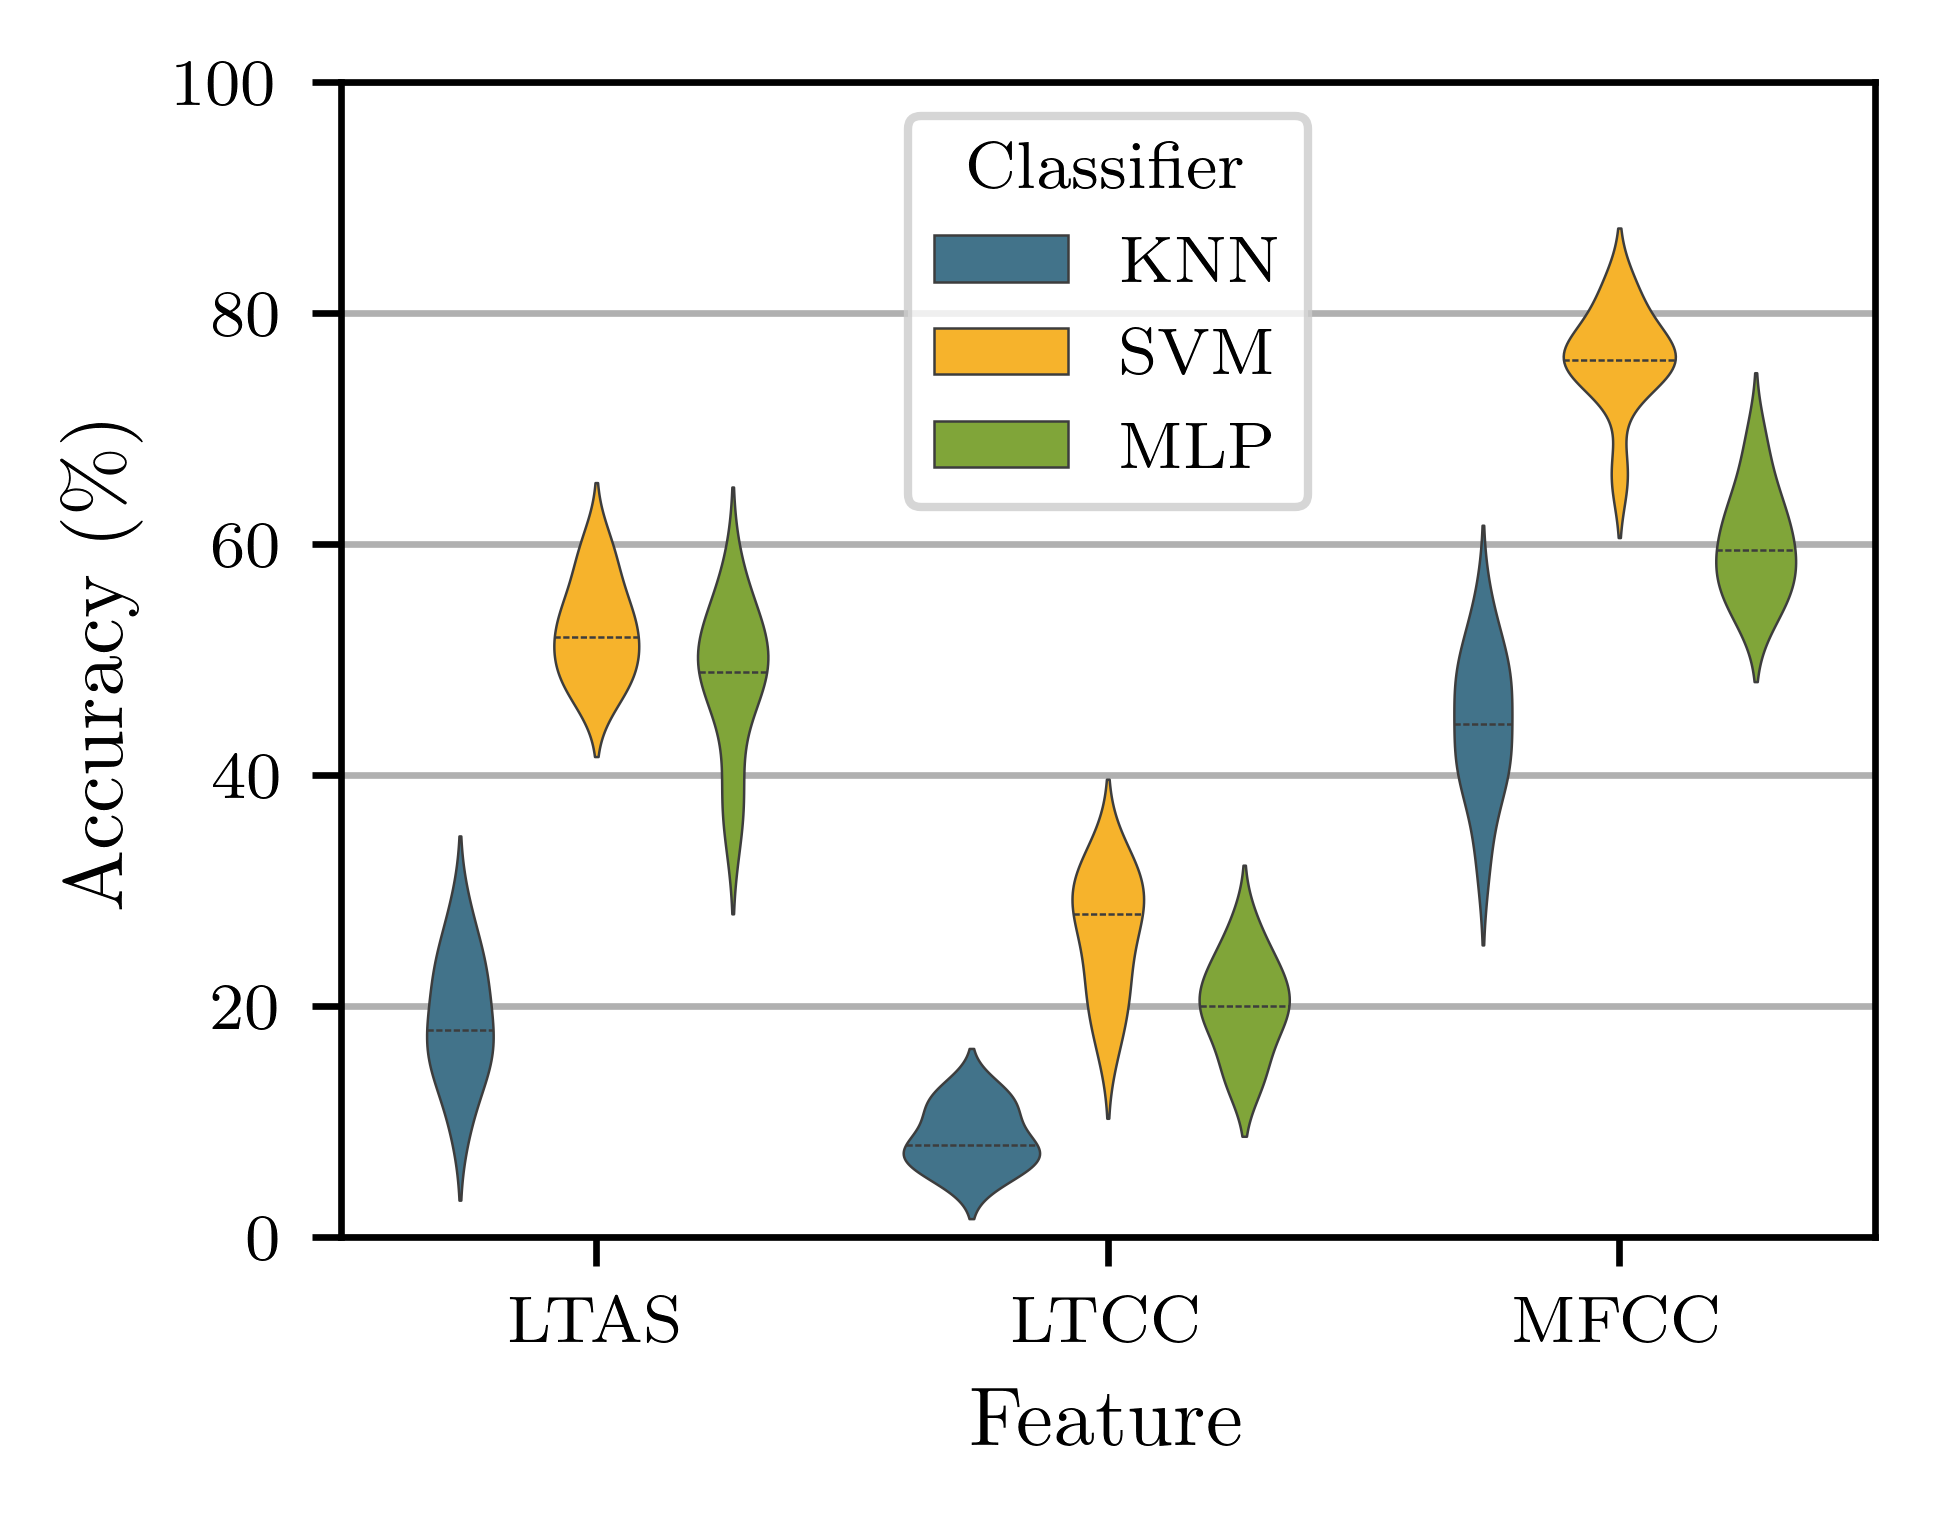
\includegraphics[width=7.8cm]{figures/accuracy-bilbao.png}
    % }
  }
  \caption{Cross-validation accuracy, Bilbao dataset.}
  \label{fig:accuracy-bilbao}
\end{figure}

\begin{figure}[!ht]
  \centerline{
    % \framebox{
      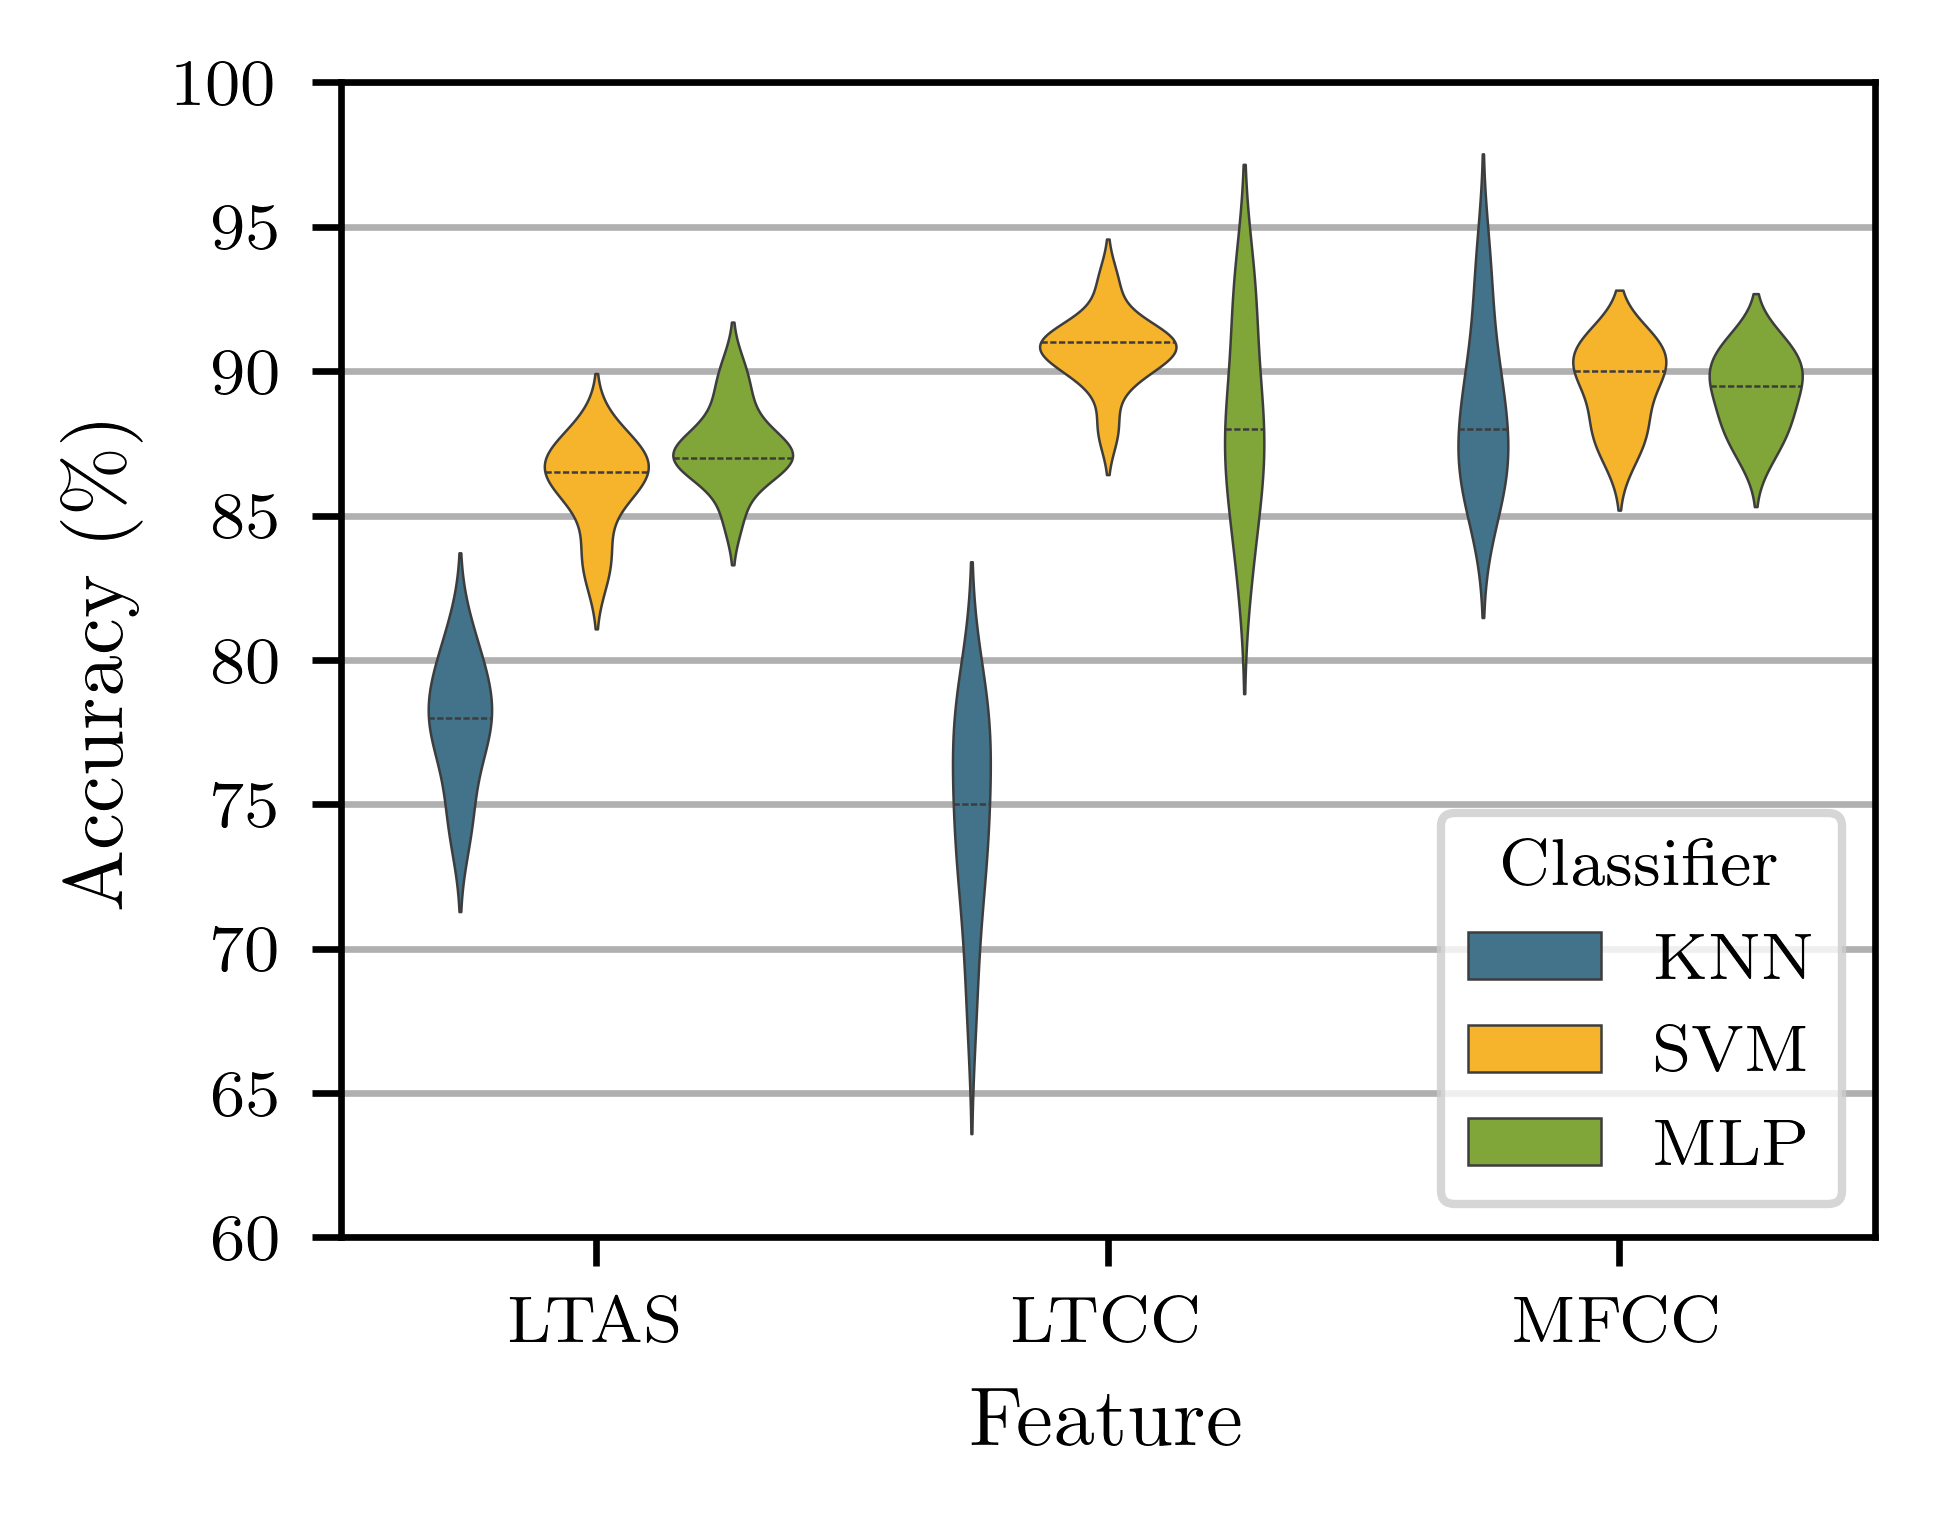
\includegraphics[width=7.8cm]{figures/accuracy-cnsm.png}
    % }
  }
  \caption{Cross-validation accuracy, CNSM dataset.}
  \label{fig:accuracy-cnsm}
\end{figure}

\noindent On the CNSM dataset, all combinations of classifiers and features achieve comparable accuracy. In contrast, with the Bilbao dataset, which is both smaller and involves a larger number of classes, the selection of appropriate features and classifiers significantly impacts performance.
We observe that MFCCs consistently deliver the best results, regardless of the classifier used. This suggests that MFCCs are the most effective features for distinguishing between violins, while taking into account variations in the playing styles of individual violinists.
Optimal performance was observed when using MFCCs with an SVM classifier. This model utilized audio recordings downsampled to a 10kHz sampling rate, retained $60$ MFCC coefficients, and employed a linear kernel in the SVM algorithm. In the rest of this paper, this model is referred to as "SVM-MFCC".

\subsection{Influence of the training data}
In this section, we use the fine-tuned SVM-MFCC model to assess the influence of training data on classification results. We focus solely on the CNSM dataset, better suited for this specific investigation due to the longer recording durations and the diversity of musical excerpts.

\subsubsection{Influence of the number of players and excerpts per player}
To understand the impact of both the number of violinists and the number of excerpts per violinist in the training data, we designed an experiment varying both parameters.  First, $20\%$ of the data was held out for testing.  Next, for systematically varied numbers of violinists ($n$) and excerpts per violinist ($m$), we trained our SVM-MFCC model using randomly selected subsets. The performance of the model was then measured on the fixed test set. The resulting accuracy values, for different ($n$, $m$) pairs, are presented as a matrix in Figure \ref{fig:influence_n}.

\begin{figure}[!ht]
  \centerline{
    % \framebox{
      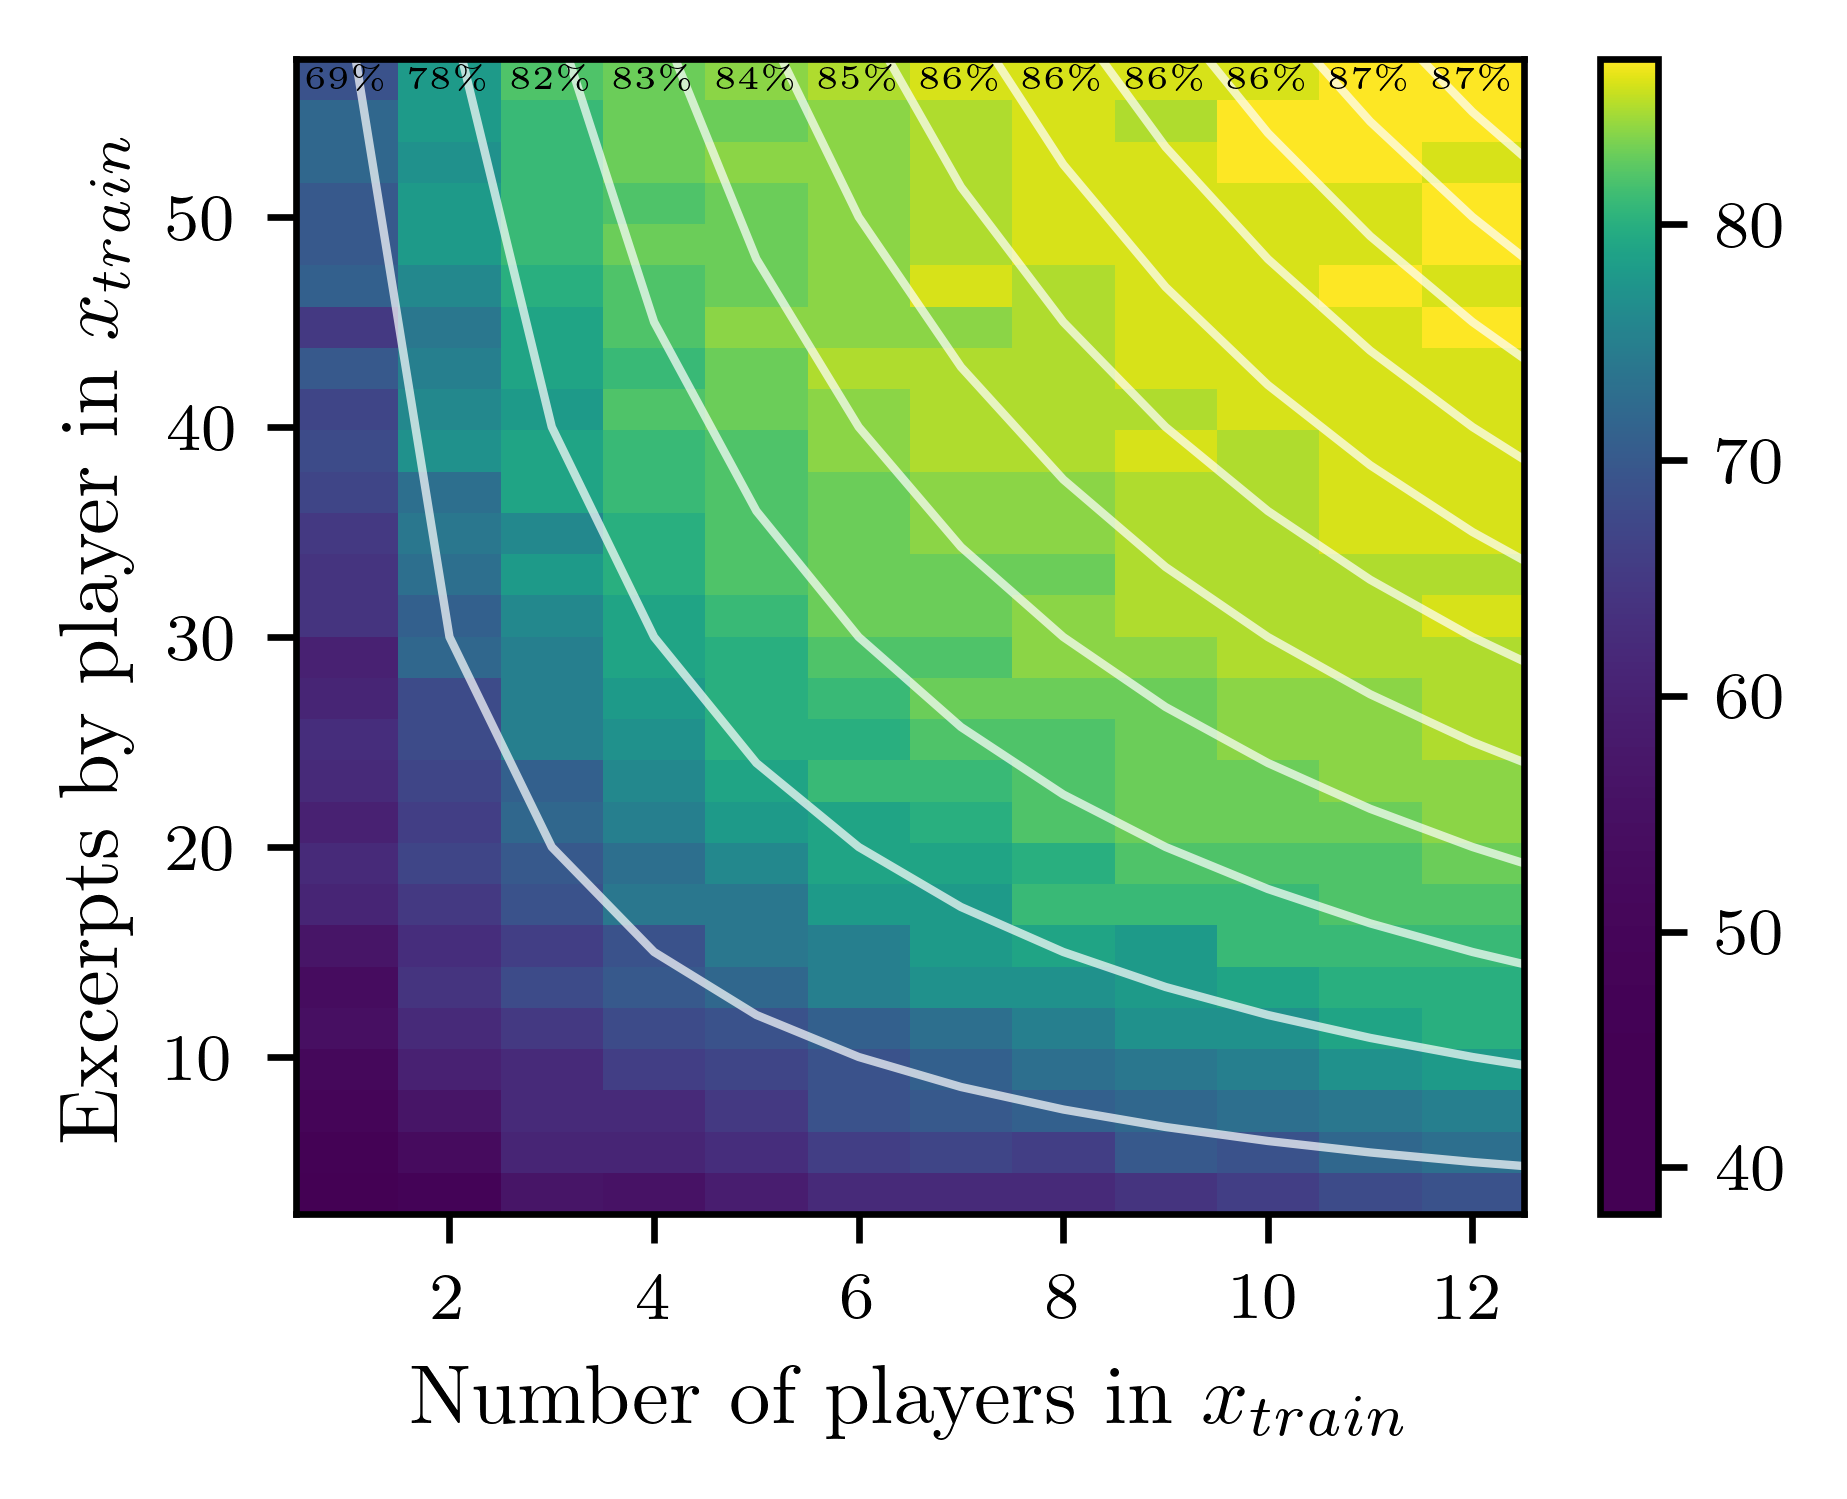
\includegraphics[width=7.8cm]{figures/matrix.png}
    % }
  }
  \caption{Test accuracy (\%) of our baseline model for random training data subsets of $n$ violinists and $m$ excerpts per violinist. The white isolines represent fixed training-set sizes.}
  \label{fig:influence_n}
\end{figure}

\noindent We observe that generally, accuracy increases with both the number of players and the number of excerpts per player. While optimal performance (87\% accuracy) was achieved when both the number of players and the number of excerpts per player were high (more than 10 players, 50 excerpts per player), moderate performance (70\% accuracy) could be reached with different trade-offs, such as using data from many players with fewer excerpts each, or fewer players with many excerpts each (as shown by the accuracy along the white lines). If achieving moderate performance is sufficient, the specific balance between the number of players and excerpts per player can be chosen based on practical constraints.

\subsubsection{Influence of the musical excerpt type}
To assess the impact of different excerpts on the accuracy, we trained our SVM-MFCC model using only recordings of the same type for training, while keeping $20\%$ of the data for testing. 
%Figure \ref{fig:influence_excerpts} highlights how the choice of the excerpt influences classification accuracy, \textcolor{red}{for two cases: in the case "same as training", the model was tested only on data from the training set that corresponded to the same excerpt on which our model was trained; in the case "different", the model was tested on all the other data of the training set.}
Figure \ref{fig:influence_excerpts} compares accuracy in two scenarios: (1)~``same as training", where the model was tested only on data from the training set that corresponded to the same excerpt on which our model was trained, and (2)~ ``different", where it was tested on all other excerpts.

 \begin{figure}[!ht]
  \centerline{
    % \framebox{
    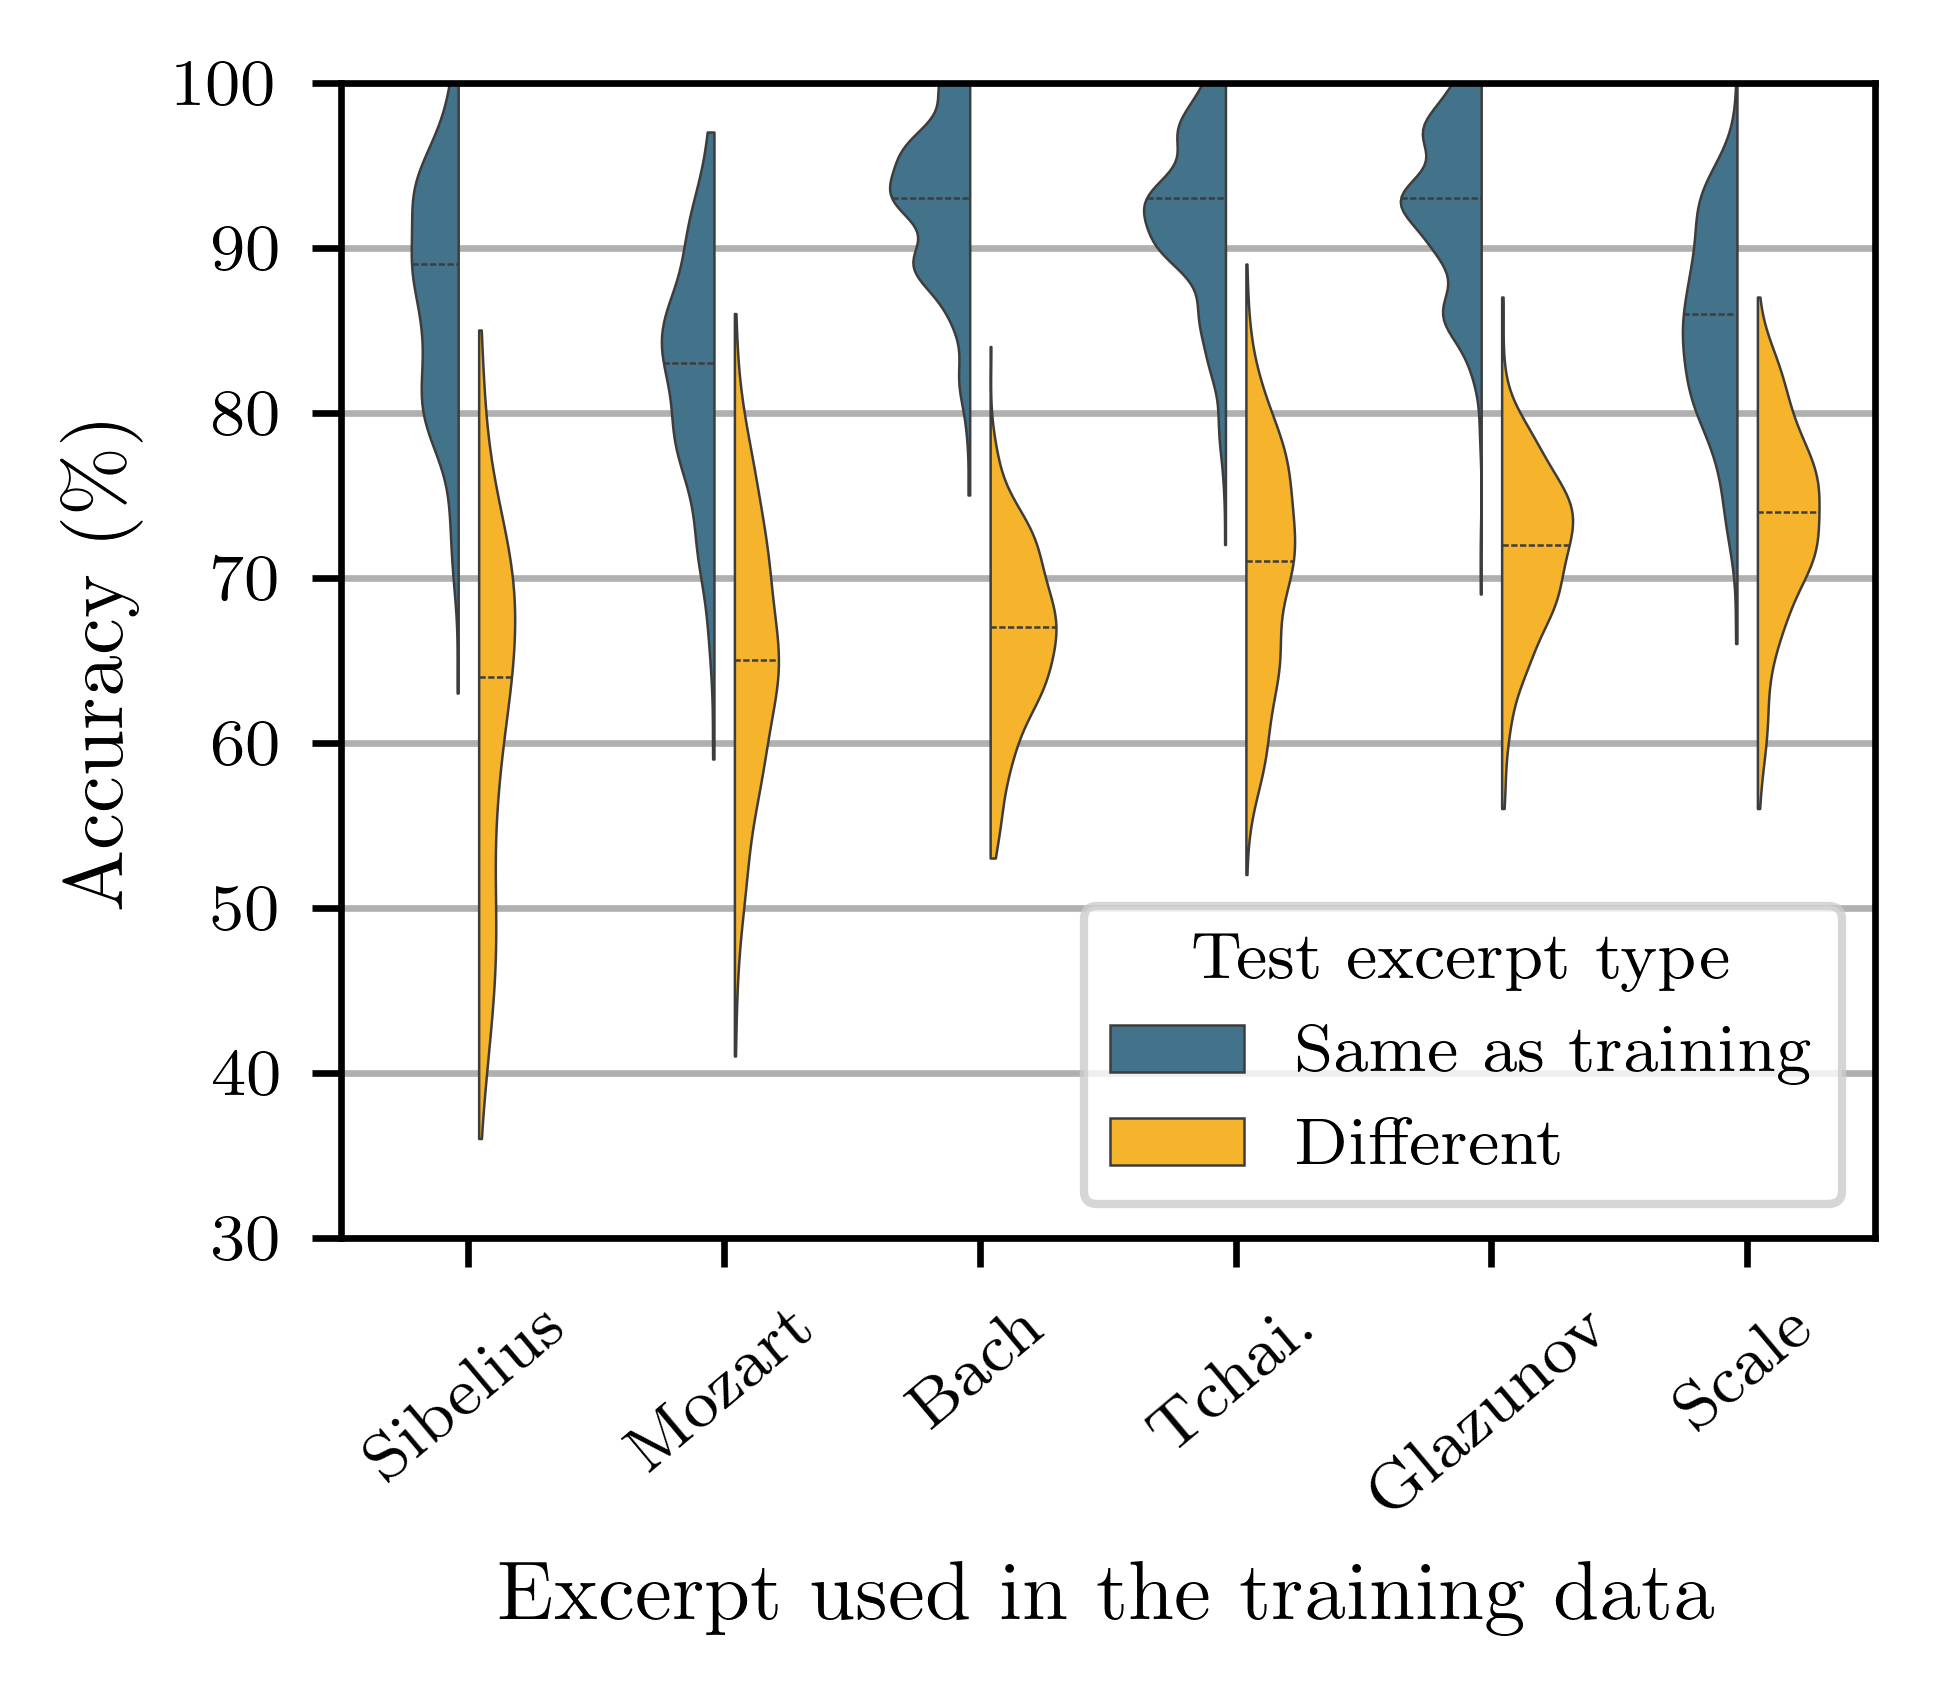
\includegraphics[width=7.8cm]{figures/accuracy-vs-excerpt.png}}
  % }
  \caption{Violin plots of the test accuracy obtained with a SVM-MFCC model using different excerpts as training data. CNSM dataset.}
  \label{fig:influence_excerpts}
 \end{figure}

\noindent Figure 4 shows that, unsurprisingly, the case "same" leads to better accuracy than the case ``different". Moreover, while the accuracy is little influenced by the type of excerpt in average in both cases, the standard deviation is larger for Sibelius and Mozart, in particular for ``different". This can be explained by the fact  that these excerpts cover -- mostly for Mozart and entirely for Sibelius -- the upper-end of the register. It thus appears that using Scales, Glazunov, and Tchaikovsky recordings are better candidates for such classification task.

\section{Conclusions}\label{sec:conclusions}
Few studies have addressed the problem of identifying individual violins based on their sound. Furthermore, the limited existing research often relies on datasets where not all violins are played by all musicians involved in the study.
Utilizing two purpose-built datasets to address this limitation, and through comparison of various features and machine learning algorithms, this study confirms the feasibility of individual violin identification. Additionally, it provides practical guidelines for selecting the number of violinists and the types of excerpts to record.
Future work will focus on exploring how MFCCs can explain perceptual evaluations of violin timbre by listeners.

\section{Acknowledgements}
This research was supported by Collegium Musicæ. We are grateful to Vincent Lostanlen for his valuable feedback.

\bibliography{references.bib}

\end{document}
